%Chapter 3 - Case studies of retro computing projects
%	What does the retro computing revival project productization process look like?
%	What risk and challenges are assosiated with a retro computing revival project?


\chapter{Case studies of retro computing projects}
\label{Chapter3}
This chapter forms a body of knowledge on retro computer revival projects that are attempting to produce a new product. This is achieved through a series of case studies into several computer projects. Each case study extracts the process that was taken in releasing a new product to market. The case studies also highlight any challenges the projects faced during the productisation process. For each case study there is a brief description of the product and the team behind it. Any information about the productisation process or challenges faced during that process is recorded. From this record, a list of the process steps is extracted, as well as a list of challenges the project faced. The challenges are then categorised into risk types for each case study. At the end of the chapter the separate case study processes are combined into a list and then illustrated, see figure \ref{case_study_process}. The separate case study risks are combined into a risk table and ranked according to the potential damage they could cause. The ranking is based off the following definitions:
\begin{enumerate}
\item Negligible 	- Slight time delay or cost on project.
\item Marginal 		- Moderate time delay or cost on project. 
\item Critical 		- Extensive time delay or cost to project.
\item Catastrophic 	- Project cannot proceed.
\end{enumerate}

%----------------------------------------------------------------------------------------
%----------------------------------------------------------------------------------------
\section{Open-source case studies}
Despite not being retro, the Arduino and Raspberry Pi where both studied because of their open-source nature and their market success. The Raspberry Pi is also influenced by retro ideas from the home computer era, such as booting straight into a programming environment as well as the creators being inspired by the BBC Micro, from the home computer era.

%%%%%%%%%%%%%%%%%%%%%%%%%%%%%%%%%%%%%%%%%%%%%%%%%%%%%%%%%%%%%%%%%%%%%%%%%%%%%%%%%%%%%%%%%%%
\subsection{Arduino}
\textbf{What is it?}\\
Arduino is a company which designs, produces and sells the Arduino range of single-board microcontrollers as seen in figure \ref{ArduinoUno3}. These are mostly 8-bit machines with 32-bit machines being introduced later and are known for being inexpensive to purchase. The Arduino company has released all the hardware designs as open-source under a Creative Commons licence. The associated IDE (Integrated Development environment) software is also open-source and Arduino also encourage and facilitate a community of hobbyist, open-source enthusiasts and professionals 
\cite{RN133}. \\

\textbf{When was it produced?}\\
The first Arduino board was designed and made available to students at the Interaction Design Institute Ivrea (IDII) in Italy in 2005. As word spread, the board quickly became popular outside of the class and Arduino boards remains hugely popular today 
\cite{RN103}.\\

\textbf{Why was it produced?}\\
It was used to help teach the students at IDII interactive design (also known as physical computing). A co-founder of Arduino, Massimo Banzi was using another commercially available microcontroller called the BASIC Stamp to teach his class prior to the Arduino board or its inspiration, Wiring being created 
\cite{RN103}. Banzi found the Stamp didn't meet his needs for teaching and it was too expensive for the students. Banzi decided to design his own microcontroller and associated IDE to create an entire platform for users to easily achieve their goals. Banzi drew heavy inspiration from another very similar project called Wiring that was also in development at IDII before and during the creation of the first Arduino board. Wiring in turn built on another related project, Processing, which provided the starting point for the IDE used in Wiring 
\cite{RN110}\cite{RN135} \cite{RN111}. \\

\begin{figure} \begin{center}
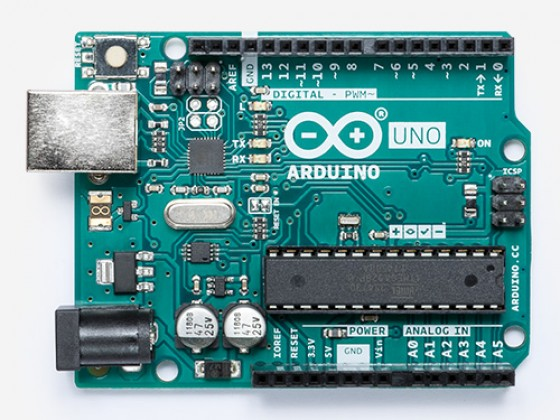
\includegraphics[width=.3\linewidth]{pics/Arduino_uno_3} 
\end{center} 
\caption{Arduino Uno Rev 3\\ \textit{\small{Picture from \url{https://store.arduino.cc/usa/}}}}
\label{ArduinoUno3}
\end{figure} 

\textbf{Process}\\
Arduino started with an idea, to create a cheap microcontroller for students and an accompanying platform to make it easy to use. From the idea stage, then a prototype was built. The prototype in this case is taken to be the microcontroller board and accompanying software Massimo Banzi and David Cuartielles developed in 2005 
\cite{RN111}. This prototype had a somewhat convoluted history, being derived from Wiring, another similar project created by a student for their thesis project 
\cite{RN110}\cite{RN111}. It's worth noting that the software or Integrated Development Environment (IDE) was (and still is) open-source and several others helped in its development, up to and after the prototype stage. Banzi and Cuartielles invited others to help with the project, an advisor Tom Igoe, a student David Mellis to help write the software and Gianluca Martino who could help facilitate the production of the board 
\cite{RN111}. After discussions with Igoe, the Arduino team decided at some point in 2005, that the target market for their product was much larger than just the students in there respectively schools. The prototype then went into a period of refinement, with the main goals of making it cheap to produce and simple to use. This included fixing some bugs in the hardware design 
\cite{RN111} and more extensive work on the IDE to included more user-friendly features. The software and hardware was also modified allow support for a cheaper chip, which is the microcontroller at the core of the Arduino board.

The Arduino team decided to produce a batch of 200 units with a prearranged agreement with two schools to buy 50 units each. The agreement meant to production run would atleast make back half of its cost, even if the other 100 boards where not sold. This reduced the risk to investors (which where Arduino team members in this case). This small production run was meant as a test to see if there was market interest in the product outside of the schools. The team then placed some paid advertisements marketing the Arduino board, as well as discussing the product with friends and colleges to spread word of mouth 
\cite{RN111}. The Arduino boards started to sell, slowly at first but it was obvious at this point that there was a market for the Arduino board.

As the Arduino is a single-board device with no case or human interface device (HID), the hardware process from working prototype to finished design was relatively simple. It consisted of just the electronic board design and parts selection with regard to price, quality and availability. A manufacture had already been found, Smart Projects, whom was owned by Arduino team member Gianluca Martino. There was also associated software actively being worked on during the period the hardware was being refined for the production run of 200 boards mentioned earlier.

The fact that Arduino creators didn't know if half of the first production run would sell and if it did, whom would be interested in it, leads to the idea that they didn't do a lot of market research before hand. The team thought of the first production run as a test to gauge market interest
\cite{RN111}. \\

\textbf{Steps Identified}
\begin{enumerate}
\item Construct a working prototype to fulfil an idea or need.
\item Decide final product features and specifications based on prototype feedback.
\item Refine prototype to remove bugs/errors and add any features that are required for the product launch.
\item Add team members as needed to help grow the project. Focus on what skills they can provide when deciding on members.
\item Self fund a small production run of the final product.
\item Place advertisements and use word of mouth to spread awareness of the product.
\item Partner with or form agreements with distributors to increase the availability of the product.
\end{enumerate} 

\textbf{Challenges faced during productisation and beyond}\\
The biggest challenge for the Arduino company was simultaneously making a profit for the company while being open-source with their products and allowing anyone to manufacture and sell them. Arduino handled this successfully, with both the designs still being open-source and the company (Arduino LLC) still trading but as it is a private company it doesn't need to publish earnings so they could not be scrutinised. The original decision to make the designs open-source, according to Banzi 
\cite{RN111} \cite{RN103}, stemmed from the realisation that IDII was running out of money and would shut within a few years, potential endangering the Arduino project. Hernando Barragán, the creator of Wiring, claims Banzi didn't have a choice and had to make it open-source. This was because Arduino used work from the Wiring and Processing projects and both of them are open-source and require any derivative to also be open-source 
\cite{RN110}. The Arduino team partnered with a manufacturer and got the first boards produced and sold for a small profit. Arduino found that as they were the first to market (with good reason) that they still sold a lot due to lack of competition, which was a possibility considering the open-source nature of the project. But when cheaper copies started being manufactured in Taiwan and China, this initially had the effect of increasing the sales through Arduino, even though there where cheaper versions available. Arduino put this down to the competition being of a lesser quality at that time 
\cite{RN113}. Arduino also charge a fee if other producers wanted to use the Arduino name. As the market matured, Arduino expected other producers and manufactures to be able to produce the Arduino boards at a cheaper price and of similar quality, which has happened. The Arduino company now focuses more on selling their expertise as the inventors, consultancy work, enabling the Arduino community and designing and selling Arduino accessories, such as 'shields', plug in devices that add extra functionality to the Arduino range 
\cite{RN113}.\\

The other big challenge Arduino faced was from legal challenges around ownership of the Arduino Trademark. In 2009, after the initial success of the Arduino boards, the co-founders decided they needed to create a company to hold all the trademarks and created Arduino LLC in the USA, as well as trademarking the name Arduino in the USA. It was decided to focus on the USA first, but one of the team members that was working on the production of the existing Arduino boards, separately registered the Arduino trademark in Italy without telling the rest of the Arduino team until 2014. In 2014, the company which held the Italian trademark and manufactured Arduino boards, Smart Projects, hired a new CEO. Smart Projects then changed its name to Arduino SRL and stopped paying Arduino LLC royalties for using the Arduino name 
\cite{RN115}. What followed was a drawn-out legal and community battle for a couple of years. In October 2016 the two parties announced an agreement to join forces and cooperate moving forward
\cite{RN116}. The schism seems to have come from two different parts of the initial group wanting to take the company in different directions, the production team wanting to keep production in Italy and the others wanting to expand into USA and China and let many other manufactures in. \\

A minor challenge the Arduino team faced was from attacks on their integrity from people that didn't like the way Banzi treated Hernando Barragán in regard to using his open-source work to create Arduino. The perceived slight was not from the use of the open-source code, which is by definition free to use, but from the fact that Banzi chose to fork and use the code without asking Barragán to be part of the Arduino team. Barragán was a past student of Banzi and they worked closely together during Barragán's creation of Wiring for his master's thesis project. Barragán also had plans to make the Wiring board compatible with cheaper microcontrollers (the chip at the core of the Arduino and Wiring boards) which is the work Banzi and team did shortly after forking the code from Wiring.\\

\textbf{Relevant useful lessons gleamed from the study}
\begin{enumerate}
\item Open source hardware can make a profit in the short term by being first to market.
\item Open source businesses can generate profit in other ways including: consultation or selling expertise of the product, licence fees for use of trademark such as Arduino \item did with their name as well as designing and producing accessories.
\item It is extremely important to keep control of trademarks and other intellectual property (IP).
\item Open-source projects encourage others to participate simple by being open, this in turn creates a community of people, these open-source communities seem to naturally converge around the original creator/s. the original creator of the Linux kernel, Linus Torvalds and the communities around Arduino and Raspberry Pi are other examples of this. The original creator/s, by being the focal point, should generally be well informed on what the community is doing, this can be leveraged by hosting community-oriented services, such as forums to share ideas and knowledge which in turn should increase the popularity of the product. \\
\end{enumerate}

\textbf{Challenges faced}
\begin{enumerate}
\item Open-source business model
\item Legal challenges to ownership of Arduino trademark
\item Attack on integrity from use of open-source work
\end{enumerate}

%%%%%%%%%%%%%%%%%%%%%%%%%%%%%%%%%%%%%%%%%%%%%%%%%%%%%%%%%%%%%%%%%%%%%%%%%%%%%%%%%%%%%%%%%%%%%%%%%%%%%%%%%%%%%%%%%%%
\subsection{Raspberry Pi}
\textbf{What is it?}\\
A cheap, open-source, single-board computer which runs a version of the Linux operating system shown in figure \ref{Raspberry_Pi}. The first version had a 32-bit processor with later version including a 64-bit processor, it's worth noting the processor chip itself is not open-source
\cite{RN99}.\\

\textbf{When was it produced?}\\
The Raspberry Pi version 1 Model B was first sold in February, 2012 for \$35, with Model A coming out soon after for 25 USD 
\cite{RN100}.\\

\textbf{Why was it produced?}\\
In 2006, Eben Upton, who grew up using a BBC Micro (from the early home computer era), had a desire to help kids learn computer science and related topics. He compared the BBC Micro on which he learned, which booted up straight into a BASIC command prompt, to modern devices children have access to, such as a tablet. He lamented that a child with a tablet is so far removed from the inner workings of the device that learning computer programming and related skills is a lot more difficult 
\cite{RN97}. To achieve his goal of helping kids learn about computers, Upton decided to make a small, cheap computer which would hopefully encourage kids to play and learn, as he did with the BBC Micro. Upton and several others formed a charity in 2009 with the purpose of advancing this agenda, called The Raspberry Pi Foundation. It wasn't until a few years later that Upton found a suitable chip for the Raspberry Pi. While working for Broadcom on the design team for the BCM2835 chip, Upton realised the BCM2835 would be perfect for the Raspberry Pi computer he had envisaged
\cite{RN97}.\\

\begin{figure} \begin{center}
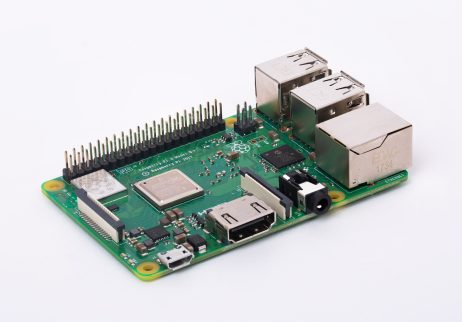
\includegraphics[width=.3\linewidth]{pics/Raspberry_Pi_3B+} 
\end{center} 
\caption{Raspberry Pi 3 Model B+\\ \textit{\small{Picture from \url{https://www.raspberrypi.org/products/}}}}
\label{Raspberry_Pi}
\end{figure} 

\textbf{Process}\\
The Raspberry Pi first started with a desire to help children engage with computers and computer topics. Eben Upton, one of the founders of the Raspberry Pi Foundation, decided the best way to achieve this was to give them access to a cheap computer that they could \"mess around\" with and learn along the way, much as he did with a BBC Micro when he was young 
\cite{RN98}. Upton built several prototypes while trying to achieve this goal. The first was built in 2006 using a microcontroller as the core and gave about the same computational power as a BBC Micro 
\cite{RN137}. Upton originally thought a highly-integrated remake of the BBC Micro would meet his goal but after discussion with like minded people, Upton abandoned this in favour of a more powerful machine 
\cite{RN98}. Upton team-up with other like minded individuals in 2009 and formed the Raspberry Pi Foundation with the stated goal to "put the power of computing and digital making into the hands of people all over the world." 
\cite{RN138}. Upton and the rest of the foundation now faced the problem that all the microprocessor available at the time where too expensive to include in a computer which needed to be cheap. It wasn't until a couple of years later that Upton found a suitable chip, the Broadcom BCM2835, a System-on-Chip (SoC), which is a complete microcomputer within a chip. In 2011, the Raspberry Pi Foundation had made a new prototype, with the BCM2835 at its core. This new prototype was shown publicly in May 2011 and received a huge amount of attention 
\cite{RN140}. In this somewhat unplanned showing, the Raspberry Pi team said they would have it finished by May 2012 and it would cost \pounds 15. This self-imposed deadline put some pressure on the team to finish by their publicly stated date.  

Over the few months the prototype design was refined, with the goal of trying to keep the board within \$35 USD. During this process several features where cut to save costs 
\cite{RN98}. Upton also embarked on a campaign to secure parts at a cheap as a possible price 
\cite{RN98}. A version of the Linux OS, designed specifically for the Raspberry Pi, was also in development 
\cite{RN98}.

Once the team had the designs for the final product agreed upon, they originally planned to make 1000 unit in the first production run to gauge the market
\cite{RN139} but after the May 2011 showing received so much attention, they revised the initial run to 2,000 units 
\cite{RN98}. The funds for the original production came from donations from the trustees of the Raspberry Pi Foundation 
\cite{RN142}. The Raspberry Pi team then had to find a manufacturer and ended up finding an outfit in China which could make the raspberry at a decent price 
\cite{RN98}. Not long after securing this initial run in 2011, the raspberry pi team realised they had more demand for units than they could secure funds to manufacture, they estimated 10,000 units would need to be made for the launch. To help solve this problem, the Raspberry Pi team partners with two large companies right before the product launch, Element14 and RS. They both agreed to distribute and manufacture the Pi, so the Raspberry Pi team pivoted at this point to becoming a designing and licensing business and not a manufacture of the Raspberry Pi 
\cite{RN98}. This partnership secured worldwide distribution and manufacturing channels, something the Upton is very proud of as he says it let the Raspberry Pi grow a lot faster 
\cite{RN98}.\\

\textbf{Steps Identified}
\begin{enumerate}
\item Construct a working prototype to fulfil an idea or need. This prototype is taken as the first with a Broadcom chip, shown publicly in May 2011.
\item Form foundation or other body to hold licenses and other IP.
\item Add team members as needed to help grow the project. Focus on what skills they can provide when deciding on members.
\item Decide final product features and specifications based on prototype feedback.
\item Refine prototype to remove bugs/errors and keep of end product cost down. Develop software needed for launch, OS and applications.
\item Get agreements for parts at acceptable prices from suppliers.
\item Launch website and have online presence, try to generate awareness through media.
\item Self fund a production run of the final product, 2000 units.
\item License out product to larger companies which can make and distribute the product better and faster
\end{enumerate} 
 
\textbf{Challenges faced during productisation}\\
The Raspberry Pi productisation process seems to have avoided most major problems, how much of this can be attributed to Upton waiting for a chip that suited the project is hard to decipher, but it most definitely helped. Whether waiting for a suitable chip is a challenge or not depends on the project.
The Raspberry team announced a release date before the final product was ready, this added a lot of pressure during that window to meet their self imposed deadline but may have helped push the project along at a faster pace 
\cite{RN97}. 
The Raspberry Pi was delayed in the first production run due to compliance laws in Europe around electronic interference compliance. The Raspberry Pi needed to be tested for electronic interference but the creators didn't realise this until it was too late to avoid delays 
\cite{RN98}. The Foundation wanted to keep the cost of a board to \$35 as they believed it would be critical to achieving their goal of allowing as many people as possible to afford one. To keep the cost down, Upton had to cut several features during the development phase 
\cite{RN98}. Upton also embarked upon an aggressive campaign to secure parts at low cost 
\cite{RN98}.\\

\textbf{Relevant useful lessons gleamed from the study}
\begin{enumerate}
\item Open source hardware can be incredibly popular. 
\item Check relevant laws and seek expert advice early as possible to avoid delays in production.
\item Keeping the cost down can greatly increase market size and device uptake. \\
\end{enumerate}

\textbf{Challenges faced}
\begin{enumerate}
\item Regulatory compliance
\item Strict product criteria on cost
\end{enumerate}

%----------------------------------------------------------------------------------------
%----------------------------------------------------------------------------------------
\section{Retro revival project case studies}
These case studies look at a group of products that are inspired by 8-bit computers from the home computer era mentioned in \ref{sec: Early home computer era}. Two of the biggest names from that time, Spectrum and Commodore are both reproduced in modern revival projects which are studied in this section. These projects are retro revival and 8-bit so they are perfect for case studies.

%%%%%%%%%%%%%%%%%%%%%%%%%%%%%%%%%%%%%%%%%%%%%%%%%%%%%%%%%%%%%%%%%%%%%%%%%%%%%%%%%%%%%%%%%%%
\subsection{Sinclair ZX Spectrum Vega}
\textbf{What is it?}\\
The Sinclair ZX Spectrum Vega is a game console inspired by the ZX Spectrum (another hugely popular home computer from the early home computer era \ref{sec: Early home computer era} which was released in the United Kingdoms in 1982 by Sinclair Research. The ZX Spectrum Vega comes preloaded with 1000 games, most of which where written for the original ZX Spectrum. It swaps the full keyboard of the original for a directional thumb pad and 9 rubber buttons as shown in figure \ref{Spectrum_Vega}. It has the endorsement of Sir Clive Sinclair, the founder of Sinclair Research. The Vega was created by Retro Computers and uses a hardware design created for the project and has a microcontroller at its core and custom-built software to allow it to play all games written for the ZX Spectrum 
\cite{RN119}.\\

\textbf{When was it produced?}\\
The Vega was released in April 2015, following a successful crowd-funding campaign on Indiegogo, a crowd-funding service. It cost 100 pounds at launch but is no longer produced or sold by Retro Computers as they have run into financial and legal troubles relating to another product, the Vega+ and was recently wound up 
\cite{RN120}.  \\

\textbf{Why was it produced?}\\
The Sinclair ZX Spectrum Vega was a commercial endeavour. \\

\begin{figure} \begin{center}
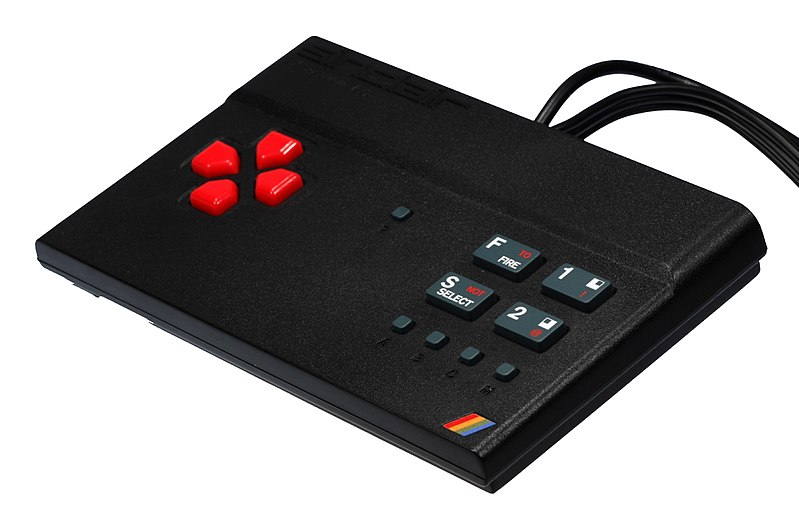
\includegraphics[width=.3\linewidth]{pics/Spectrum_Vega} 
\end{center} 
\caption{Sinclair ZX Spectrum Vega, a game console with 1000 preloaded games inspired by the ZX Spectrum from 1982. \\ \textit{\small{Picture courtesy of Marco Tangerino}}}
\label{Spectrum_Vega}
\end{figure} 

\textbf{Process}\\
\label{Vega process}
The Sinclair ZX Spectrum Vega first came to public attention due to a crowd-funding campaign launched by it creators Retro Computer (RCL) on Indiegogo in 2014. The campaign was intending to raise the capital needed manufacturer the first production run of the Vega. The campaign was successful, raising 149\% of their intended goal or \pounds 155,682. Retro Computers Limited (RCL) claimed in the campaign that the design was complete already and that RCL had agreements in place to use the Sinclair brand as well as the rights to use 1,000 games that would be shipped with the Vega. The terms of the agreement with the games rights holders was that RCL can distribute the games on the Vega but for each Vega sold a donation must be made to a charity for 10\% of the Vega purchase price. To secure the rights to use the Sinclair name, Paul Andrews, the managing director of RCL at the time, reached out to Sir Clive Sinclair to seek his approval, which was forthcoming with the provision that David Levy be able to join RCL and provide oversight on behalf of Clive. Once the crowd-funding campaign had secured funding, RCL went about finding a manufacturer and in January 2015 they announced they had formed an agreement with SMS Electronics Ltd to manufacture the Vega. Later the same month RCL announced that they have received suggestions on how to improve the Vega from various parties and they would be implementing two of them: adding extra buttons and adding an hardware interface and ability to upgrade the software. RCL also noted that the Vega had passed the required ECM (Electromagnetic compatibility) test in June 2015. Later the same month RCL posted on the Indiegogo campaign page that the first production run of the Vega had been complete but they could not legally send them to backers yet as they first needed a PEGI (Pan European Game Information) age rating. RCL announced that the first batch of Vegas where sent to backer on the 7th of August 2015.\\

\textbf{Steps Identified}
\begin{enumerate}
\item Construct a working prototype to fulfil an idea or need, in this case it was basically feature complete and finished, this included the electronics design as well as the tooling and case designs and software. 
\item Form agreement with relevant license or rights holders to use their IP.
\item Launch crowd-funding campaign to raise capital for first production run.
\item Find and form agreement with manufacture/s to produce product.
\item Refine prototype based on community suggestions.
\item Organise to have product tested as required by relevant laws. The Vega needed to pass an ECM test and a PEGI age rating test.
\item Launch website to sell product and have an online presence.
\item Send out finished product to backers.
\end{enumerate} 

\textbf{Challenges faced during productisation}\\
The Indiegogo campaign was successful, raising 149\% of the funding goal 
\cite{RN119}. 
Retro Computers launched a crowd-funding campaign offering a product to backers which wasn't complete yet, since this campaign, there has been a successful legal challenge that states that this type of agreement is a sales contract and such they are legally obliged to deliver the product regardless of problems that could arise before the product is complete 
\cite{RN122}. This ruling came from legal action against the Indiegogo crowd-funding campaign for next iteration from Retro Computers the Sinclair ZX Spectrum Vega Plus console. So by offering a product to backers in a crowd-funding campaign, Retro Computers exposed themselves to extra risk and it may have been better to word the crowd funding campaign differently to avoid this or just not offer the product to backers at all but rather sell it to them cheaper once it is finished (if it gets finished).\\

\textbf{Relevant useful lessons gleamed from the study}\\
Crowd-funding campaigns can be useful to raise capital but offering a as-yet unfinished product to backers exposes the campaign founders to an amount of risk in that they legally have to deliver the product and there may be unforeseen costs and challenges in producing it.\\

\textbf{Challenges faced}
\begin{enumerate}
\item Crowd-funding campaign to deliver product that had not been finished
\end{enumerate}

%%%%%%%%%%%%%%%%%%%%%%%%%%%%%%%%%%%%%%%%%%%%%%%%%%%%%%%%%%%%%%%%%%%%%%%%%%%%%%%%%%%%%%%%%%%
\subsection{Spectrum Vega+}
\textbf{What is it?}\\
The follow up of the Sinclair ZX Spectrum Vega mention earlier. It is, like it predecessor, inspired by the Sinclair ZX Spectrum and also has the endorsement of Sir Clive Sinclair, although it is reported he has very little to do with the actual running of Sinclair Research 
\cite{RN123}. The Vega Plus is a hand-held console with its own screen and internal battery as well as the ability to output its display to a TV, although this feature couldn't be made to work in a review of the Vega Plus 
\cite{RN117}. The Vega+ has a microcontroller at its core which provides the computational power 
\cite{RN143}.\\

\textbf{When was it produced?}\\
In July 2018, Retro Computers sent out a number of Vega Plus consoles to backers. No other Vega Plus consoles have been produced.\\

\textbf{Why was it produced?}\\
Like its predecessor, the Vega Plus was a commercial endeavour. \\

\begin{figure} \begin{center}
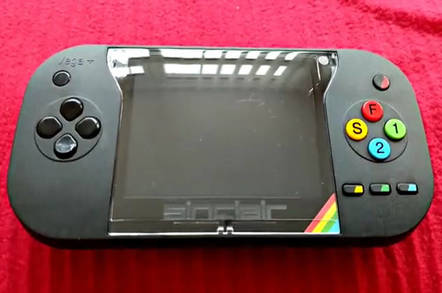
\includegraphics[width=.3\linewidth]{pics/Spectrum_vega_plus} 
\end{center} 
\caption{Sinclair ZX Spectrum Vega Plus console, the poorly received culmination of a tumultuous crowd-funding campaign  \\ \textit{\small{Picture courtesy of Craig Wootton}}}
\label{Spectrum_Vega_Plus}
\end{figure} 

\textbf{Process}\\
The Spectrum Vega+ was the next product offered by Retro Computers Limited (RCL) after the Spectrum Vega, mentioned above in section \ref{Vega process}. Like the Vega, the Vega+ used a crowd-funding campaign on Indiegogo to raise capital to fund the first production run of 2,500 units and prepare for the second production run 
\cite{RN143}. When the campaign was launched on 15th February 2016, RCL claimed they had a working prototype of the Vega+ and supplied video evidence to back up this claim 
\cite{RN145}\cite{RN143}. The campaign closed on the 27th of March 2016 having successful reached its target; it raised 366\% of the target or \pounds 512,790. 
But not long after the end of the campaign, two of the directors of RCL resigned citing "irreconcilable differences" between them and the remaining directors
\cite{RN146}. One of the directors, Chris Smith, was also the creator and owner of the firmware which was created to run the Vega+, when he left he took the rights to use them with him and refused RCL the rights to use it in the upcoming Vega+. This proved to be a difficult situation for RCL to recover from while under the leadership of the sole remain director, Dr David Levy. RCL eventually released a small number of the Vega+ consoles to no more than 400 of the over 4,500 backers of the campaign after Indiegogo threatened to send debt collectors after RCL to recover the funds unless backers received a Vega+ 
\cite{RN147}. RCL has now been wound-up by creditors demanding payment and no more Vega+ consoles are ever likely to be made, leaving thousands of backers without the product they paid for and hundreds of thousands of pound unaccounted for 
\cite{RN120}\cite{RN148}. By almost any metric it can be said the Vega+ project was an abject failure and such the process they used will be of little value. \\

\textbf{Steps Identified}
\begin{enumerate}
\item Construct a working prototype to fulfil an idea or need.
\item Launch crowd-funding campaign to fund first production run and prepare for second run
\item Lose rights to use prototype from first point, forced to remake the firmware because of this.
\item Add team members as needed, Levy brought in two new directors after Smith and Andrew resigned.
\item Make promises to backers about the imminent delivery of the product but don't deliver, this happened numerous times after the end of the crowd-funding campaign, which was during the development of the Vega+ with the new firmware.
\item Release a very small number of units to some backers after multiple threats of debt collectors from Indiegogo and legal challenges from backers trying to receive refunds.
\item Wind-up business and stop communicating with backers.
\end{enumerate} 

\textbf{Challenges faced during productisation}\\
The Vega Plus crowd-funding campaign and subsequent unkept promises of delivery from Retro Computers has been reported as one of the worst crowd-funding disaster stories ever. With the Indiegogo campaign raising 366\% of the funding goal, over half a million pounds (over \$900,000 AUD). Following on from a successful campaign with proven results and the backing and involvement of home computer era luminaries Sir Clive Sinclair and designer Rick Dickinson. As well as a working prototype and completed designs for the Vega Plus and the expertise within Retro Computers to finish the product. It would be fair to give the project a fair chance of success in finishing the Vega Plus and delivering them to backers. What actually occurred can not be called successful by any metric and it is amazing to compare to very poorly received results with the potential at the beginning of the campaign.

The first and biggest challenge faced was that very early into the campaign, two of the directors of Retro Computers resigned including the CTO Chris Smith who was the designer of the Vega Plus prototype and held the rights to it, which he took with him when leaving the company. This left Retro Computers having to start from scratch with the hardware design and firmware for the Vega Plus after already promising over 4000 backers they would deliver a Vega plus. This in turn lead to delays. Retro Computers made many failed promises of delivery to the backers during this time, cause much angry from the backers. Several legal actions followed, most notable a backer took Retro Computers to court claiming they broke a contract of sale with him over the Vega Plus 
\cite{RN122}. Interestingly Indiegogo's terms explicitly state that any rewards to backers are perks or gifts but the court ruled differently in part because the receipt to the backer for his pledge stated his order for a Vega Plus had been received and this formed a contract of sale between Retro Computers and the backer (not Indiegogo). Retro Computers now legally had to deliver the Vega Plus or refund the backers money, but reports from the times show Retro Computers was haemorrhaging money and didn't have a working prototype. Retro Computers then lost the rights to use the 1000 games that where included on the Vega, this was due to the license holders, Sky (Media?) withdrawing support due to the ongoing controversy surrounding the Vega Plus which was already well behind its delivery date with no progress to show. Retro Computers eventually managed to scrape together a barely functional console using a open-source spectrum emulator called FUSE (Free Spectrum Emulator) and a collection of 8? games all made by a single developer that was closely associated with Retro Computers and the Vega Plus project. Retro Computers claims they sent out 400 Vega Plus consoles to backers, with no word of when the rest are coming. One concerned backer did some investigating and found the number of consoles sent out to be closer to 50. Following this, Retro Computers was wound-up by an ex-director of Retro Computers, while functioning as the director of another company, claiming the Retro Computers owns them money. So as it stands Retro Computers is closed, no more Vega Plus (or indeed Vega) consoles are likely to be made and a large amount of money has gone missing with very little to show for it. There is ongoing legal actions against various directors of Retro Computers about these issues.\\

\textbf{Relevant useful lessons gleamed from the study}
\begin{enumerate}
\item Keep control of needed intellectual property needed for the project, form agreements with holders of IP for there use in the project before making any promises of delivery of product. 
\item Don't do anything to jeopardize any current contracts, such as Retro Computers did to lose the backing of Sky and thus the ability to include the games they had promised.
\item Be honest with backers and investors as to the state of the project, this is especially true for crowd-funding backers as these campaigns generally involve a large number of people.
\item Don't make claims or promises that cannot be kept in reasonable circumstances.
\item Crowd-funding campaigns offering products to backers can possible be seen to be a contract of sale between the backers and the campaign founders. This in turn forces the campaign founder to act according to the law regarding a contract of sale, including such things as refunds and guarantees of delivery.
\end{enumerate}

\textbf{Challenges faced}
\begin{enumerate}
\item Loss of agreement for use of intellectual property
\item Crowd-funding campaign to deliver product which is not yet completed 
\item Use of 3rd party intellectual property 
\end{enumerate}

%%%%%%%%%%%%%%%%%%%%%%%%%%%%%%%%%%%%%%%%%%%%%%%%%%%%%%%%%%%%%%%%%%%%%%%%%%%%%%%%%%%%%%%%%%%
\subsection{ZX Spectrum Next}
\textbf{What is it?}\\
The ZX Spectrum Next is a fully functional 8-bit computer that closely emulates the Sinclair ZX Spectrum from 1982. It achieves this by emulating the Spectrum in a FPGA board. The maker claim they will release the hardware design as open-source once it is complete. The case design is by Rick Dickinson the celebrated case designer of the original Spectrum series.

\textbf{When was it produced?}\\
It is currently under production. The Next is the focus of a Kickstarter crowd-funding campaign, which was launched in April 2017 and gave the original delivery date as January 2018. The campaign was well funded, raising £723,390 from over 3000 backers.

\textbf{Why was it produced?}\\
A commercial enterprise.

\begin{figure} \begin{center}
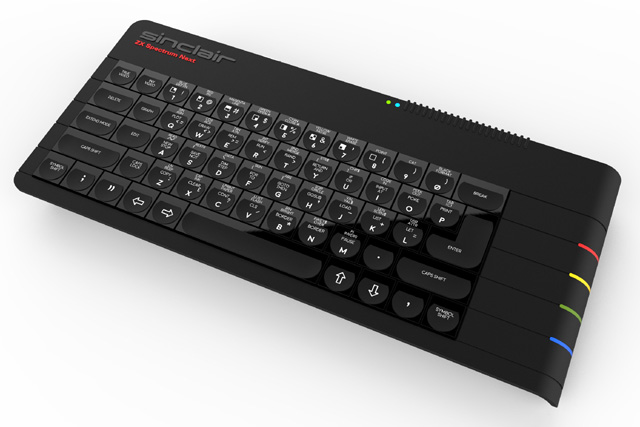
\includegraphics[width=.3\linewidth]{pics/spectrum_next} 
\end{center} 
\caption{ZX Spectrum Next, intended to be a fully functional iteration of the Sinclair ZX Spectrum. The makers claim it will be fully compatible with all software written for the original Spectrum \\ \textit{\small{Picture from \url {https://www.specnext.com/about/}}}}
\label{Spectrum_Next}
\end{figure} 

\textbf{Process}\\
The ZX Spectrum Next is an innovation of the ZX Spectrum from 1982. It is currently in the production phase of development after successfully raising \pounds 723,390 on a crowd-funding campaign on Kickstarter. When the crowd-funding campaign was launched on April 23rd 2017, the Next team had a working prototype with most of the hardware design finished, they did add some features later when the crowd-funding campaign was so successful 
\cite{RN151}. They also had CAD designs for the case and keyboard completed before the campaign 
\cite{RN149}. With the capital raised from the crowd-funding campaign they intend to fund the first production run of the Spectrum Next. Not long after the end of the campaign which was on the 23rd of May 2017, The Next team released a website to act as a Next portal to house information for the community including hardware, software, drivers and firmware for the Next 
\cite{RN154}. In April 2018, the Next team promised to have fortnightly updates on the Kickstarter page, this was in response to backers requests 
\cite{RN155}. They also mentioned they have nearly decided on a manufacturer for the keyboard and the case 
\cite{RN155}. The electronic manufacturer had been decided earlier 
\cite{RN151}. The Next team also mentioned in April 2018, their plans for the box and manual that would be included with the Next 
\cite{RN151}.\\

\textbf{Steps Identified}
\begin{enumerate}
\item Construct a working prototype without case or keyboard. 
\item Create finished CAD drawings of the keyboard and case.
\item Launch crowd-funding campaign to raise funds for the first production run.
\item Refine prototype to add new features, made possible by the crowd-funding campaign raising more than expected. 
\item Regularly make updates to backers informing them of the progress made or problems faced.
\item Launch website portal to house community information and have online presence outside of Kickstarter.
\item Decide on manufacturers or keyboard, case and electronics.
\item Have manufacturers produce sample products for testing and quality control.
\item Adjust CAD drawing and make any other changes needed based on samples from manufactures.
\item Secure components for manufacturing e.g. RAM, resistors, capacitors etc. 
\item Finish work on manual and box designs and content.
\item Agree to start final production run with manufacturers. 
\end{enumerate} 

\textbf{Challenges faced during productisation}\\
The makers have had trouble with the mechanical function of the keyboard which has delayed production while they try to fix the issue. The last given expected delivery date was the 2nd quarter of 2019. There is also evidence the firmware the Next is running is still under development. The Next team also mentions problems with the exchange rate, as the value of the pound had been falling compared to the US dollar during the production period, this made it hard for them to source all the components within their budget 
\cite{RN159}. The Spectrum Next team also had to consider the effects of Brexit 
\cite{RN157}. The chosen manufacturer of the case unexpectedly the project unexpectedly due to the manager resigning and the new manager not considering the project worthwhile for their business 
\cite{RN158}. This caused some delay as the team had to find a new case manufacturer, the Next team was also worried about incurring storage costs because of this. If the keyboards where finished before the case then they would have to go into storage, costing the Next team extra money. It turned out that due to delays with the keyboard, this wasn't an issue. Another issues faced was due to a stretch goal (a stretch goal is an additional goal for the crowd-funding campaign that was above the first goal of funding the production), the inclusion of RAM sockets that would allow new RAM to be added without the need to solder, caused some problems as the devices are not in common usage any more and thus hard to buy or get manufactured. They did eventually find a manufacturer which still had the parts to make the sockets and that also agreed to make a small run for the Next 
\cite{RN159}. \\

\textbf{Relevant useful lessons gleamed from the study}
\begin{enumerate}
\item The time taken for quality control and testing of the buttons and keys can escalate and endanger the entire project.\\
\end{enumerate}

\textbf{Challenges}
\begin{enumerate}
\item Keyboard mechanism design issues
\item Crowd-funding in currency other than US dollars made it difficult to source components
\item Brexit
\item Supplier failure to deliver
\item Sourcing old component 
\end{enumerate}

%%%%%%%%%%%%%%%%%%%%%%%%%%%%%%%%%%%%%%%%%%%%%%%%%%%%%%%%%%%%%%%%%%%%%%%%%%%%%%%%%%%%%%%%%%%
\subsection{C64 Mini}
\textbf{What is it?}\\
A mini form-factor game console inspired by the Commodore 64. It also is a fully functional Commodore 64-like computer which can be control via a USB connected keyboard (not included). It has a non-functional keyboard and a functional joystick which connects to the console via a cable. The console connects to a TV to display in 720p resolution. The C64 Mini came pre-loaded with 64 game written for the Commodore 64, it also has the ability to load game ROMs from a USB flash stick. It was funded through a crowd-funding campaign on Indiegogo 
\cite{RN124}, the campaign was intended to raise funds to pay design work on the case and keyboard as well as pay for the first production run. The creators of the Mini are Retro Games, they originally planned on releasing a full-size and hand-held console (with build-in screen) form factor but during the production period, on the 28th of April 2017, they pivoted to focus on the C64 Mini form-factor with the full-size version to follow later 
\cite{RN160}. It's interesting to note that the resigned directors of Retro Computers (the company behind the unpopular Vega Plus campaign), Paul Andrews and Chris Smith (they resigned before the company went off the rails) are involved, as well as Darren Melbourne who worked on the C64 DTV 
\cite{RN127}. The Mini has a ARM SoC at its core, which runs a software emulation of the C64 
\cite{RN160}. Retro game have stated that they will open-source the designs as much as possible once the production is complete, currentley they have not even though the C64 Mini has been released but the full-size version is still under production\\

\textbf{When was it produced?}\\
Released in the first quarter of 2018.

\textbf{Why was it produced?}\\
A commercial endeavour. 

\begin{figure} \begin{center}
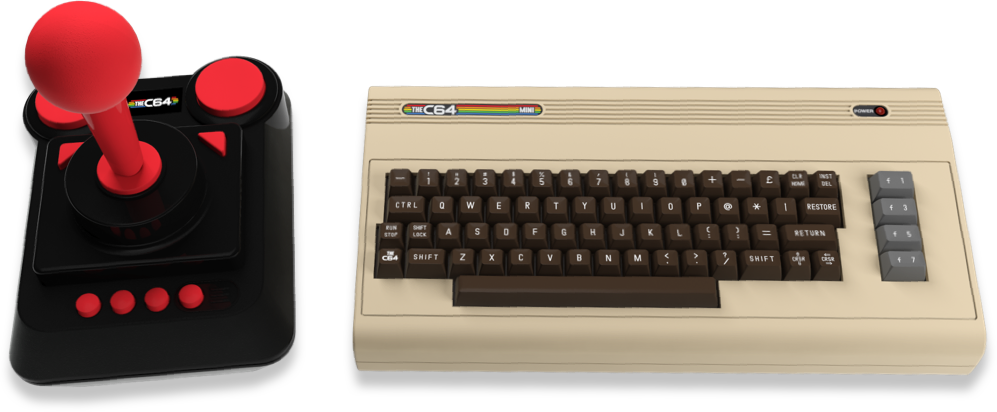
\includegraphics[width=.3\linewidth]{pics/C64_mini} 
\end{center} 
\caption{C64 mini\\ \textit{\small{Picture from \url {https://retrogames.biz/thec64-mini/}}}}
\label{C64_mini}
\end{figure}

\textbf{Process}\\
Retro Games didn't have a functional prototype at the campaign launch, it wasn't shown till August 2016, running on preproduction hardware. After campaign had finished, Retro Games tried to partner with a manufacturer and distributor to get the c64 worldwide retail release. Retro Games secured extra funds missing from crowd-funding campaign as well as focusing on c64 Mini first at partners request. Retro Games worked on circuit design for 3 form-factors of the C64 range, as well as CAD designs for case and keyboard and component selection. Retro Games also sought agreements from game developers to use their games in the Mini during production period. \\

\textbf{Steps Identified}
\begin{enumerate}
\item Launch crowdfunding campaign.
\item Create functional prototype on preproduction hardware.
\item Find partner to invest, manufacture and distribute.
\item Re-evaluate with partner best business direction (Retro Games focused on C64 Mini form-factor)
\item Secure game rights.
\item Finish circuit designs for final product and component selection and sourcing. Design with compliance in mind.
\item Create CAD drawings of case and keyboard.
\item Create manual and box design.
\item Test pre-production units and make amendments to product or processes as needed.
\item Start production run and send to backers.
\item Retail release.
\end{enumerate} 

\textbf{Challenges faced during productisation}\\
The crowd funding campaign did not meet the target goal of \$150,00 USD, reaching 67\% of the target or \$100,611 USD. Retro Games delayed their production schedule because of this, but ultimately they reached and agreement with an international distributor and manufacturer which allowed them to continue without seeking further funding
\cite{RN125}. This collaboration with the aforementioned partner also lead Retro Games to rethink their plans, they pivoted to focus on the C64 mini version entirely and get that complete first before moving to the full size version.

\textbf{Relevant useful lessons gleamed from the study}\\
Regular communication with backers is important for a successful crowd-funding campaign, this includes listening to them and responding to their concerns and queries. Paul Andrews and Chris Smith must have been aware there could be potential backlash over their involvement in the Vega Plus quagmire (they where both directors of Retro Computers when the Vega Plus campaign was launch but left a few months later). They remained honest (to the best of my knowledge) about the situation and who they where and probably of most importance, gave regular weekly updates to backers describing progress made and relevant news as well as progress pictures whenever possible. They also, on several occasions, publicly answered specific questions from backers, which would go a long way to alleviating fears and concerns from the backers about a repeat of the Vega Plus campaign.  \\

\textbf{Challenges}
\begin{enumerate}
\item Failure to reach crowd-funding goal
\end{enumerate}


%%%%%%%%%%%%%%%%%%%%%%%%%%%%%%%%%%%%%%%%%%%%%%%%%%%%%%%%%%%%%%%%%%%%%%%%%%%%%%%%%%%%%%%%%%%
\subsection{C64 DTV}
\textbf{What is it?}\\
A single-board Commodore 64 clone housed within a joystick, comes preloaded with 30 games. It was, unsurprisingly from the name, inspired by the Commodore 64. It features an ASIC (Application-specific Integrated Circuit) at its core 
\cite{RN129} and has the possibility of after market modification due to exposed solder points on the board
\cite{RN126}. The C64 DTV was born from another project, the C-One which was also created by the DTV's designer, Jeri Ellsworth. The C-One is a single-board C64 clone made using FPGA technology.\\

\textbf{When was it produced?}\\
First released in 2014 with version 1, which support only NTSC Broadcasting Television standard. Version 2 came out in 2015 with additional PAL support\\

\textbf{Why was it produced?}\\
A commercial endeavour. \\

\begin{figure} \begin{center}
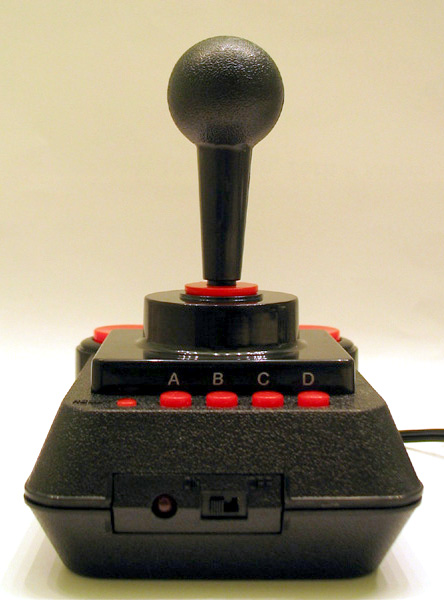
\includegraphics[width=.3\linewidth]{pics/C64_DTV} 
\end{center} 
\caption{C64 DTV or C64 Direct-to-Television \\ \textit{\small{Picture courtesy of Christian Wirth}}}
\label{C64_DTV}
\end{figure}

\textbf{Process}\\
The C64 DTV was an innovation of an earlier product, the C-One. The C-One is a single-board C64 clone that uses FPGA technology. The DTV is a smaller version of the C-One which fits into a accompanying joystick case, as shown in figure \ref{C64_DTV}. The DTV is aimed at letting users play Commodore 64 games, of which 30 where included. The DTV does not support the ability to load game ROMs after purchase but it is possible with some after-market modifications 
\cite{RN161}.\\

\textbf{Steps Identified}\\
\begin{enumerate}
\item Construct a working prototype to fulfil an idea or need, the prototype here is taken as being the prototype which lead to the C-One. 
\item Partner with others that can help turn the prototype into a product, the C-One.
\item partner with others that have skills to develop a games console based off the C-One.
\item Design and create the C64 DTV case including joystick and PCB based off the C-One.
\item Form partnership to market and distribute product.
\end{enumerate} 

\textbf{Challenges faced during productisation}\\
The C64 DTV was derived from another similar product, the C-One. Jeri Ellsworth designed an enhanced version of the Commodore 64 as a way to teach herself about programming FPGAs. Ellsworth then partnered with Individual Computers to turn her FPGA design into a product, the C-One. Other manufactures and retailers saw potential in the C-One and asked Ellsworth if she would consider making a smaller version that would fit in a joystick, with a focus on enabling users to play games, shown in figure \ref{C64_DTV}. Unfortunately it seems very little was published about the process from turning the C-One into the C64 DTV or from earlier efforts to complete the C-One.\\

\textbf{Relevant useful lessons gleamed from the study}\\
\begin{enumerate}
\item Retro games can sell quite well, nostalgia is a powerful incentive.
\item Extra features included in the device can help boost sales, these can be features that are not normally available but the device can be hacked or modified by the user to make them available. There are reports of user buying the DTV simply to access the C64-like computer running at its core.
\item ASICs are a technology that could be applied to this area.
\item There is a larger market for consoles that focus on playing games than other uses of a 8-bit computer.
\end{enumerate}

\textbf{Challenges}
\begin{enumerate}
\item None identified
\end{enumerate}

%------------------------------------------------------------------
%------------------------------------------------------------------
\section{Retro computing productisation: process}
This section consolidates the processes collected from the case studies above. A discussion of any interesting or useful conclusions drawn from the comparison follows.\\

\subsection{Combined process from case studies}
The following is a combination of the processes identified in the case studies. The steps that are common to all or most case studies are included, as well as two possible funding models.\\

\textbf{Combined Process}
\begin{enumerate}
\item Construct a working prototype.
\item Control IP.
\item Research relevant laws and regulatory obligations and make design changes to accommodate as well as budgeting for any costs likely to be incurred in future testing.
\item Decide final product features and specifications based on prototype feedback.
\item Add team members as needed to help grow the project. Focus on what skills they can provide when deciding on members.
\item Create CAD designs for case, keyboard and any other parts that need to be custom made for the final product.
\item Launch crowd-funding campaign or raise funds through private investors or businesses for first production run.
\item Refine prototype to remove bugs/errors and add any features that are required for the product launch.
\item Launch website to give a web presence and foster a community.
\item Find manufacturer for electronics, plastics (case, keyboard etc.) and source components.
\item Partner with or form agreements with distributors to increase the availability of the product and market the product.
\end{enumerate} 

Most of the discovered processes from the case studies agreed on an outline of a process to productisation, which is listed above. One of the points of difference between the processes identified in the individual case studies is how much of the design work was complete before announcing the release of the product to the public, either through a crowd-funding campaign or other method. The decision to announce earlier in the design process may be due to businesses constraints, if the project is in need of funds to continue, then announcing early may be worth the increased risk. The risk in announcing early is due to uncertainty in several factors: currency changes, law changes such as 'Brexit', unknown costs for manufacturing and design changes. The other main point of difference was where to use a crowd-funding service to raise capital or to rely of private investor and/or business partnerships or a mixture of both. With regard to a crowd-funding campaign, it has been proven to be possible to be successful but a successful campaign, such as the Next, Vega and Vega+ had several common features. Successful in this context relates solely to the campaign's fund raising effort, not the end result generated from the funds. The 3 campaigns named, all had a lot of information about the product as well as a working prototype to show in video. All 3 campaigns also posted regular updates as well as responding to community requests and/or concerns.

It is hoped that the process described here will be useful for new retro computing projects and form a basis for further research in this area. \\

\begin{figure} \begin{center}
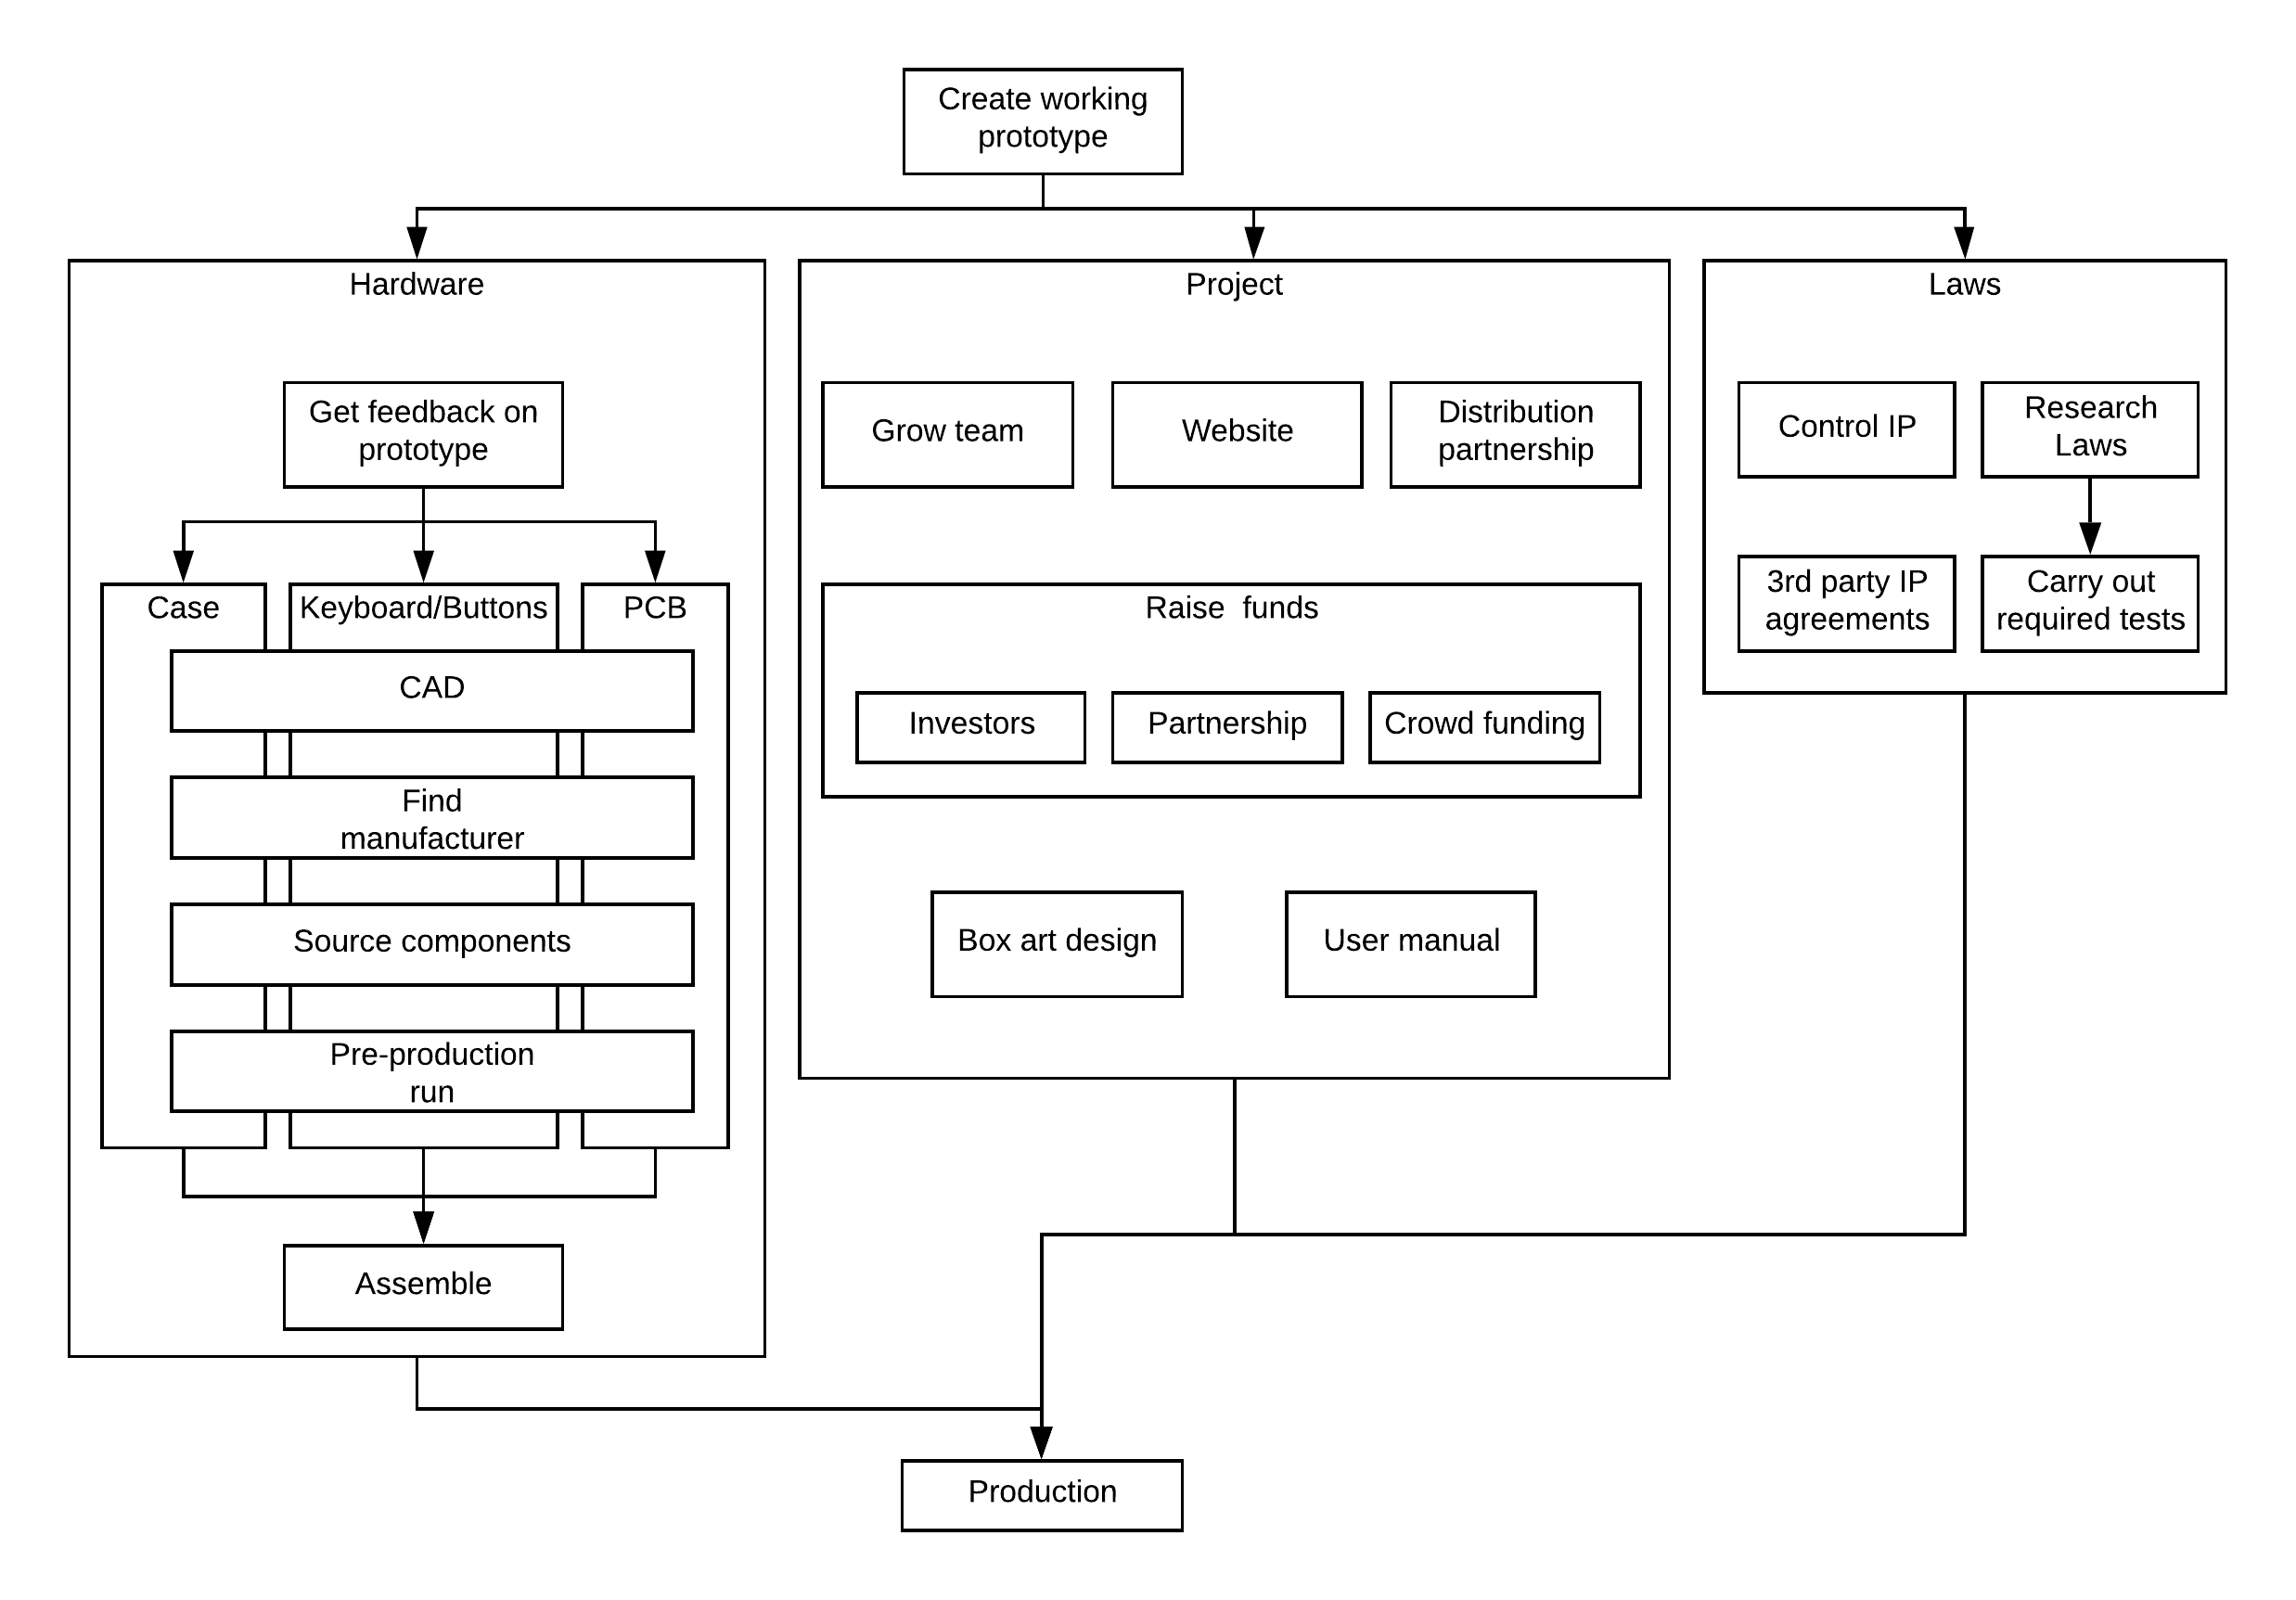
\includegraphics[width= 1\linewidth]{pics/case_study_process} 
\end{center} 
\caption{Retro computer productisation process. Small rectangles are tasks, larger rectangles are task areas.}
\label{case_study_process}
\end{figure} 

%------------------------------------------------------------------
%------------------------------------------------------------------
\section{Retro computing productization: associated risks}
One aim of the case studies was to gain information about the type of challenges a retro computer project may face in creating a new product. That information is consolidated in this section. This is achieved by categorising the challenges into risks.


\subsection{Combined risks from case studies}
The risk identified in the case studies are combined and ranked to produce a list of risks that are relevant to a retro computer project. It is intended these risks be considered along side the typical project risks, such as time, money and technical ability, as examples. For each identified risk, a description of the risk is given. The factors which affect the potential damage and likelihood are also discussed. \\

\subsection{Laws and regulations}
\textbf{Regulatory compliance}\\
Several case studies ran into problems around complying with required laws or regulations needed to enter the market with a new product. The Raspberry Pi experienced some delays because the team didn't think their product needed to undergo electronic emissions testing when in fact it did. By the time the team realised this it was too late to avoid any delay and still undergo the testing. While the Raspberry Pi team did only experience a slight to moderate delay of a week or two, the risk has still been rated at catastrophic because if Raspberry Pi had not passed the test as the product was, there was a good chance the Raspberry Pi project would have failed.\\

\subsection{Brexit-like event}



\subsection{Project constraints}
\textbf{Strict product criteria on cost}\\
The Arduino and Raspberry Pi both aimed their products to be very cheap to purchase. In the case of the Raspberry Pi this caused some considerable changes to the product during the prototyping and design phase. Several features where cut and the Raspberry Pi team had to embark on an aggressive series negotiations with parts suppliers. This risk is given the catastrophic rating as the Raspberry Pi team was so set on the price point they stated publicly before the product was complete, that if the team hadn't been able to achieve their vision within that price, the project had a chance of being abandoned.\\
  
\subsection{Crowd-funding}

\subsection{Crowd-funding: Contract of sale}

\subsection{Crowd-funding: Currency}

\subsection{Crowd-funding: Failure to meet goal}
\textbf{Crowd-funding to deliver product that doesn't exist yet}\\
This risk is associated with all of the case studies that used crowd-funding to generate funds. The risk to the project comes from backers of the campaign starting legal proceedings against the campaign founders. The legal preceding are due to backers not receiving what they believe they are entitled to, namely the product offered to backers of the campaigns. This could be because the product was never delivered or delivered late or there where significant changes to the product that it no longer resembles what the backers saw when they backed the campaign. The most visible example of this is the Vega Plus project and it's precedent-setting legal troubles. This risk was given a catastrophic rating as the legal trouble could easily have stopped any of the crowd-funded projects in the case studies from being complete. Although it is arguable that if it got to the state where backers where successfully suing the campaign founders for failure to deliver, then there's a good chance the project was already in trouble.\\

\subsection{Sourcing old components}
\textbf{Sourcing old component}\\
The use of old components can bring increased risk due to lack of supplies, manufacturing techniques or tools and increased cost due to less volume of parts. Old components is taken to mean components that are no longer frequently used to build modern electronic devices. Some retro computing projects like to incorporate old components because they where used on the inspiration of their projects. The Spectrum Next experienced this problem, it's inspiration, the ZX Spectrum used ICs connected via sockets for RAM. This allowed the RAM to be changed without the use of tools. This risk was categorised as catastrophic because depending on the circumstances it could stop a project completely. In the case of the Next it was only a marginal cost to the project, but depending on the component in question, the risk could be catastrophic.\\

\subsection{Use of 3rd party intellectual property}
\textbf{Use of 3rd party intellectual property}\\
This risk is associated with all of the retro revival projects as they all used or attempted to use 3rd party games with their software. Every project studied handled this very well except for one stand out project failure, the Spectrum Vega Plus. The risk to projects comes from many, if not all retro revival projects need 3rd party software to run on their machines, this is because they want the same or similar experience as that which inspired the project. A Commodore 64 revival project would not be as successful in the market place without retro Commodore 64 software to run on it, as an example of the problem. Another aspect to consider is sometimes the ownership of retro software is ambiguous, making forming agreements for its use impossible. This leaves some retro software in murky territory regarding legal use. \\

\textbf{Failure to meet crowd-funding funding goal}\\
Many retro revival projects in the case study used crowd-funding to raise funds for their first production run. If the funds could not be raised via crowd-funding, many of the projects would have been stopped.\\

\textbf{Project member leaving and taking their IP }\\
This risk is most obvious from the Vega Plus case study in which the CTO left with their design of the prototype shown in the crowd-funding videos. This risk is dependant on the amount of IP used in the project and more importantly who holds ownership or who has agreement to use aforementioned IP. If the IP holder is an individual and their is no agreement in place to use the IP, or if the agreement allows the withdrawal of aforementioned IP without good reason, then the risk is increased. Inversely, if an entity associated with the project, such as the Raspberry Pi foundation, is the entity which holds ownership of the IP, then the risk is significantly reduced. \\

\textbf{Legal challenges to ownership of intellectual property}\\
The Arduino case study highlighted a case where the Arduino team had to endure legal challenges against the use of the Arduino trade mark. This didn't effect the initial productisation of the Arduino boards, as it occurred much later in the business's time line. But the same thing could easily effect a project earlier and is worth considering from the beginning of a projects life cycle. In Arduino's case, they chose to only register the trademark in the USA

\subsection{Open-source business}
\textbf{Open-source business model}\\
The Arduino project is both open-source and a business trying to generate a profit. The somewhat unorthodox business model brings with it some increased risks.\\

\subsection{Loss of intellectual property}
\textbf{Supplier failure to deliver}\\
The Spectrum Vega experienced a set back when a supplier suddenly dropped their project. This risk is not unique to retro revival projects but is included because the Spectrum Next experienced a delay when a a manufacturer suddenly decided to not produce their product. The potential damage and likelihood of this event occurring is specific to each supplier and each purchase. The likelihood of this event occurring can be reduced by using reputable, established suppliers as well as undertaking due diligence into suppliers before entering into agreements. The potential damage occurred is dependant on the nature of the purchase which the supplier failed to deliver as well as the nature of the failure. If the purchase was of a high critical component that the project needs to move forward, then the potential damage can be critical. If the purchase was for an incidentals part which could be easily obtained from numerous suppliers then the potential cost would be negligible.\\

\subsection{Supplier failure}

\subsection{Open-source fair use}}

\textbf{Attack on integrity from use of open-source work}\\
The Arduino project experienced a slight challenge from certain individual that considered the way in which Banzi used the open-source work the formed the start of the Arduino project as unethical. This mainly stems from the fact that Banzi was the supervisor of a student's project that Arduino was started from. Individuals feel it was unethical to use the work without inviting the student in question to join the Arduino team. This was a very minor problem for the Arduino team in terms of lost time or increased costs. \\

\subsection{Physical production problems}

\textbf{Keyboard mechanism design issues}\\
The Spectrum Next experienced some delay due to the mechanism on he keyboard buttons.\\ 

\textbf{Crowd-funding in currency other than US dollars}\\
The Spectrum Next experienced problems arising from the decision to use English pounds as the currency to use in their crowd-funding campaign. This resulted in difficulties because most of the electronic components they had to purchase later in the productisation period where made using USD (US dollars) and the exchange also changed during that period, resulting in the Next project having less USD to spend.\\ 

\textbf{Brexit-like events}\\
Brexit is the unofficial name given to the event of the United Kingdom leaving the European Union. This is a very specific event and will not need to be considers specifically soon (as Brexit will have been finished). This Brexit event is used here to illustrate the type of large policy changes that can affect retro revival projects if there customers, partners or their team is situated in a country undergoing an event such as Brexit. In the case of Brexit, it is causing some concern for the Next team that a post-Brexit environment may have unforeseen laws and regulations they need to abide by to sell in European countries. Large scale trade wars and economic recessions are other similar large scale events that should be considered.\\

\begin{figure} \begin{center}
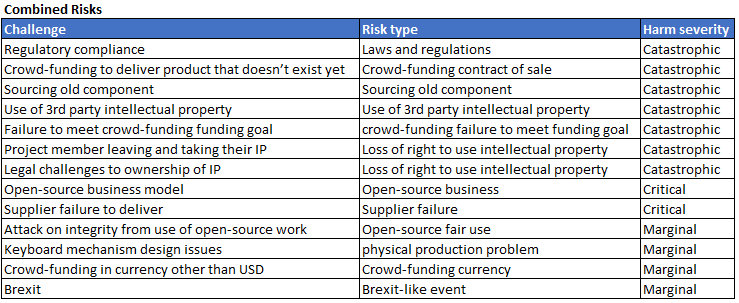
\includegraphics[width= 1\linewidth]{pics/risk_list} 
\end{center} 
\caption{Combined list of risk associated with a retro computer project}
\label{case_study_process}
\end{figure} 